Actor Model programming is selected as the top-level programming model for the workload application. Actor Models are specifically designed for parallel programming and fit the Open Event Machine API layout well. Prototyping Actor Model programs is straightforward due to available graphical tools. Actor Model rapid prototyping tool PREESM will be utilized in the experiment to build a simple version of the workload. PREESM was selected over comparable tools for the following reasons: 1. PREESM supports TMS320C6678 as a compilation target. 2. PREESM is under active development.

An actor network is constructed in PREESM that represents the video filter application. A network sketch is presented in Figure~\ref{sketch}.

\begin{figure}[h!]
\begin{center}
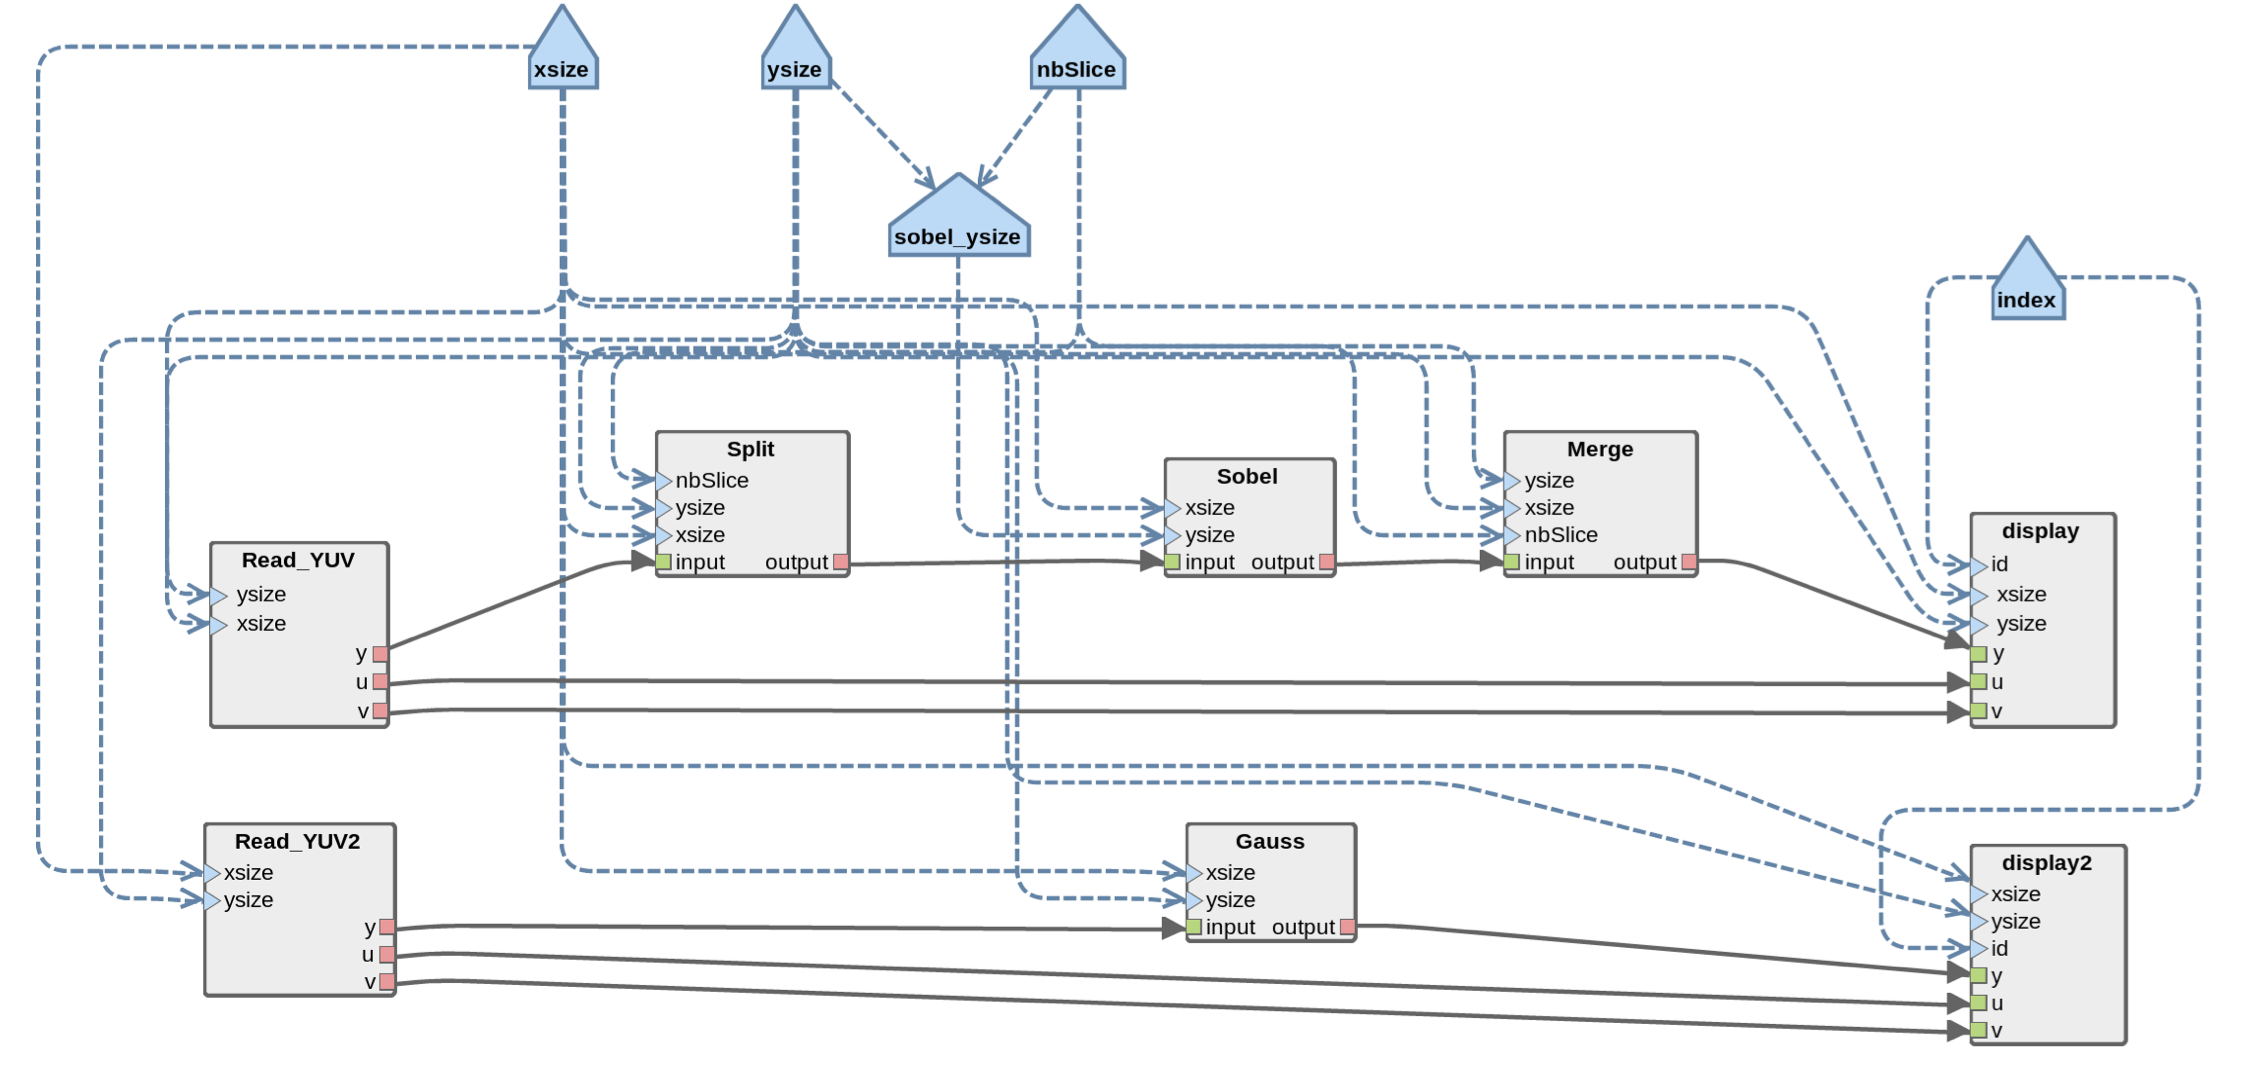
\includegraphics[width=1.3\textwidth,natwidth=2250,natheight=1090]{preesm_gauss.png}
\caption{A Sketch of The Video Filter Actor Network}\label{sketch}
\end{center}
\end{figure}

To keep the model simple and the program well analyzable all of the processing paths in the network are independent. The shared dependencies in the sketch (marked with dashed lines) are constants related to the video stream and will change in the actual application.

Each filter implemented will have its own independent processing path.

The first actors on each of the processing paths load the video frames form memory and pass them to a splitting actor. The splitting actor splits the frames to suitable number of splices to enable processing the same video stream on multiple cores. The filter actor follows the splitting actors. Partial frames filtered in the filter actor are merged in to whole frames in the merge actors. The last actors on each processing path are sink actors that collect data from the execution and frees resources.

The filter actors will be run on all cores according to manual selection before execution. The cores on which the other actors will run on are to be determined.

PREESM version 2.1.3 and Eclipse Luna Service Release 2 (4.4.2) will be used in the experiment.

\textbf{Pelcat M. et. al.} Preesm: A dataflow-based rapid prototyping framework for simplifying multicore DSP programming 10.1109/EDERC.2014.6924354
